%\documentclass{article}
\documentclass[journal,12pt,twocolumn]{IEEEtran}

% Language setting
% Replace `english' with e.g. `spanish' to change the document language
\usepackage[english]{babel}

% Set page size and margins
% Replace `letterpaper' with `a4paper' for UK/EU standard size
%%\usepackage[letterpaper,top=2cm,bottom=2cm,left=3cm,right=3cm,marginparwidth=1.75cm]{geometry}

% Useful packages
\usepackage[utf8]{inputenc}
\usepackage{enumitem}
\usepackage{multicol}
\usepackage{ragged2e}
\usepackage{amsmath}
\usepackage{amssymb}
\usepackage{graphicx}
\let\vec\mathbf
\newcommand{\myvec}[1]{\ensuremath{\begin{pmatrix}#1\end{pmatrix}}}
\usepackage{array}
\usepackage{blindtext}
%\usepackage[paperwidth=10cm]{geometry}
\usepackage{tkz-euclide}
%\usepackage{tikz}
\usetikzlibrary{
  circuits.logic,
  circuits.logic.US,
  positioning
}
\usepackage[colorlinks=true, allcolors=blue]{hyperref}

\title{Circle Assignment}
\author{Navya Valmeekam}
\begin{document}
\providecommand{\norm}[1]{\left\lVert#1\right\rVert}
\maketitle
\begin{tableofcontents}
\section{Problem}
\noindent The abscissa of the two points A and B are the roots of the
equation x2+2ax-b2=0 and their ordinates are the roots of the equation x2+2px-q=0. Find the equation and the radius of the circle with AB as diameter.\\
\\
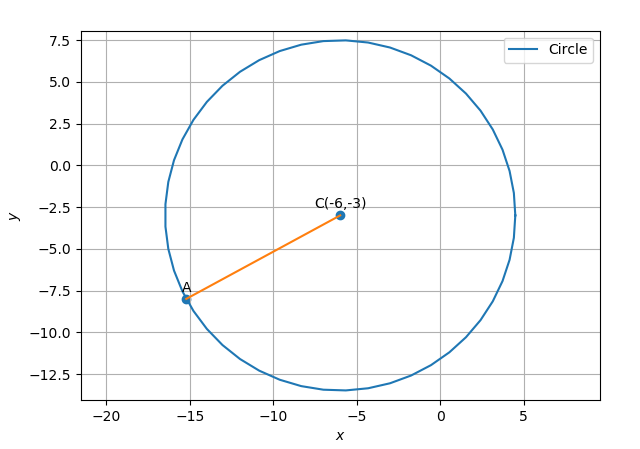
\includegraphics[scale=0.4]{circle.png} 
\begin{center}
Figure of Construction
\end{center}
\vspace{0.3cm}
\section{Construction}
\begin{center}
\begin{tabular}{|c|c|c|}
\hline
\textbf{Symbol}&{Value}&{Description}\\
\hline
\textbf{C}&$\myvec{-6 \\ -3}$&Center of the circle $C_1$\\
\hline
\textbf{r}&10.4&Radius of the Circle\\
\hline
\end{tabular}
\end{center}
%\end{abstract}
\vspace{0.5cm}
\section{Solution}
The roots of the equation $\vec{x^2+2ax-b^2=0}$ are \\
\begin{equation}
\begin{pmatrix}
\vec{x1} \\
\vec{y1}
\end{pmatrix}
=
\begin{pmatrix}
\vec{-a+\sqrt{a^2+b^2}}\\
\vec{-a-\sqrt{a^2+b^2}}
\end{pmatrix}
\end{equation}
The roots of the equation $\vec{x^2+2px-q^2=0}$ are \\
\begin{equation}
\begin{pmatrix}
\vec{x2} \\
\vec{y2}
\end{pmatrix}
=
\begin{pmatrix}
\vec{-p+\sqrt{p^2+q^2}}\\
\vec{-p-\sqrt{p^2+q^2}}
\end{pmatrix}
\end{equation}
From question point A and B becomes\\
\begin{equation}
\vec{A}
=
\begin{pmatrix}
\vec{-a+\sqrt{a^2+b^2}}\\
\vec{-p+\sqrt{p^2+q^2}}
\end{pmatrix}
\end{equation}
\begin{equation}
\vec{B}
=
\begin{pmatrix}
\vec{-a-\sqrt{a^2+b^2}}\\
\vec{-p-\sqrt{p^2+q^2}}
\end{pmatrix}
\end{equation}
Given AB is diameter so, Center C will be midpoint of A and B\\ 
\begin{equation}
\therefore \vec{C=\frac{A+B}{2}}
\end{equation}
We get,
\begin{equation}
\vec{C}
=
\begin{pmatrix}
\vec{-a}\\
\vec{-p}
\end{pmatrix}
\end{equation}
Radius of circle is given by,
\begin{equation}
\vec{r=\norm{A-C}}
\end{equation}
We get,
\begin{equation}
\vec{r=\sqrt{a^2+b^2+p^2+q^2}}
\end{equation}
From
\begin{equation}
\vec{r=\sqrt{\norm{c}^2-f}}
\end{equation}
We get,
\begin{equation}
\vec{f=-b^2-q^2}
\end{equation}
From 
\begin{equation}
\vec{C=V^{-1}u}
\end{equation}
We get, 
\begin{equation}
\vec{u}
=
\begin{pmatrix}
\vec{a}\\
\vec{p}
\end{pmatrix}
\end{equation}
\begin{equation}
\vec{x}^{\top} \vec{V} \vec{x} + \vec{2} \vec{u}^{\top} \vec{x}+f=0
\end{equation}
Substituiting u and f in standard equation of conics, we get equation of circle.\\
\end{tableofcontents}
\end{document}